% Presentazione della tesi magistrale - Luca Milanesi
% Compilare dalla cartella principale della tesi, ad esempio: pdflatex presentazione/presentazione.tex   (slide)
%                pdflatex presentazione/discorso.tex      (slide + testo del discorso)
%                pdflatex presentazione/riserva.tex      (slide + slide di riserva per le domande)
\documentclass[aspectratio=169,12pt]{beamer}

\usepackage[T1]{fontenc}
\usepackage[scaled=0.92]{helvet}
\usepackage{courier}
\usepackage{array}
\usepackage[utf8]{inputenc}
\usepackage[italian,provide=*]{babel}
\usepackage{amsmath}
% matematica come nella tesi (Libertine + newtxmath), testo in sans
\usefonttheme[onlymath]{serif}
\usepackage[libertine]{newtxmath}
\usepackage{booktabs}
\usepackage{pifont}
\usepackage{tikz}
\usetikzlibrary{arrows.meta, positioning, fit, backgrounds, calc, shapes.multipart}


% --- Aspetto ---------------------------------------------------------------
\definecolor{unimi}{RGB}{0,51,102}
\definecolor{okgreen}{RGB}{30,130,60}
\definecolor{kored}{RGB}{180,40,40}
\definecolor{dioblue}{RGB}{218,232,252}
\definecolor{diogreen}{RGB}{213,232,212}
\definecolor{dioorange}{RGB}{255,230,204}
\definecolor{diored}{RGB}{248,206,204}
\definecolor{dioblueborder}{RGB}{108,142,191}
\definecolor{diogreenborder}{RGB}{130,179,102}
\definecolor{dioredborder}{RGB}{184,84,80}
\definecolor{reqblue}{RGB}{25,85,190}
\definecolor{areafill}{RGB}{230,224,248}
\definecolor{areaborder}{RGB}{112,88,190}
\definecolor{areatext}{RGB}{78,55,155}
\usetheme{default}
\setbeamertemplate{navigation symbols}{}
\setbeamersize{text margin left=8mm,text margin right=8mm}
\setbeamercolor{frametitle}{fg=unimi}
\setbeamerfont{frametitle}{series=\bfseries,size=\Large}
\setbeamercolor{structure}{fg=unimi}
\setbeamercolor{alerted text}{fg=kored}
\setbeamertemplate{itemize items}[circle]
\setbeamertemplate{frametitle}{\vspace{3mm}\insertframetitle\par\vspace{-2.5mm}{\color{unimi!35}\rule{\textwidth}{0.6pt}}\par}
\setbeamertemplate{footline}{\hfill{\scriptsize\color{gray}\insertframenumber\,/\,\inserttotalframenumber}\hspace{8mm}\vspace{3mm}}
\setbeamerfont{note page}{size=\footnotesize}
\addtobeamertemplate{note page}{\setlength{\parskip}{1.2ex}}{}
% \ifdefined\CONDISCORSO\setbeameroption{show notes}\fi
\setbeameroption{show notes}

\newcommand{\ok}{\textcolor{okgreen}{\ding{51}}}
\newcommand{\ko}{\textcolor{kored}{\ding{55}}}
\newcommand{\msg}[1]{\vfill{\centering\color{unimi}\bfseries #1\par}}
\newcommand{\ctxbox}[2]{{\footnotesize\bfseries #1\par}\vspace{2pt}#2}

\title[Scheduling Policy-Driven di Task in Kubernetes con Vincoli di Protezione dei Dati]{Scheduling Policy-Driven di Task in Kubernetes\\con Vincoli di Protezione dei Dati}
\author{Luca Milanesi}
\date{}

\begin{document}

% ===========================================================================
\begin{frame}[plain, noframenumbering]
\centering
\begin{minipage}{\dimexpr\textwidth-12mm\relax}
\begin{minipage}[c]{0.15\linewidth}
\includegraphics[width=\linewidth]{immagini/loghi/unimi}
\end{minipage}\hspace{5mm}%
\begin{minipage}[c]{0.75\linewidth}
{\small Università degli Studi di Milano\\
Corso di Laurea Magistrale in Informatica}
\end{minipage}

\vspace{8mm}
{\color{unimi}\fontsize{16}{21}\selectfont\bfseries Scheduling Policy-Driven di Task in Kubernetes\\ con Vincoli di Protezione dei Dati\par}
\vspace{8mm}

\begin{minipage}[t]{0.48\linewidth}
\textbf{Candidato}\\ Luca Milanesi\\ {\small Matricola 55053A}
\end{minipage}\hfill
\begin{minipage}[t]{0.48\linewidth}
\textbf{Relatore}\\ Prof.ssa Sara Foresti\\[2mm]
\textbf{Correlatore}\\ Prof.ssa Pierangela Samarati
\end{minipage}

\vspace{6mm}
{\footnotesize\color{gray} Anno Accademico 2025-2026}
\end{minipage}

\note{Buongiorno a tutti, sono Luca Milanesi e la mia tesi riguarda lo scheduling di task guidato da politiche con vincoli di protezione dei dati, implementato in Kubernetes.}
\end{frame}

% ===========================================================================
\begin{frame}{Introduzione: contesto generale}
\begin{center}
\includegraphics[height=0.68\textheight]{immagini/esempio.jpg}
\end{center}
\vspace{-1mm}
{\centering\small Enti esterni sottomettono i propri task al cluster dell'organizzazione che detiene i dati.\par}

\note{Partiamo dal contesto generale. Spesso, chi possiede dei dati vuole renderli \textbf{utilizzabili ad altri senza cederli direttamente}: ad esempio un consorzio di ospedali che mette dati clinici a disposizione di gruppi di ricerca esterni.

L'idea è quindi \textbf{portare la computazione dove si trovano i dati}. Come in figura, enti esterni sottomettono i task, e l'organizzazione li esegue sui nodi del proprio cluster che ospitano i dataset, senza che gli enti conoscano la struttura del cluster o decidano dove eseguirli.}
\end{frame}

% ===========================================================================
\begin{frame}{Dove si colloca la tesi}
\begin{center}
\vspace{2mm}
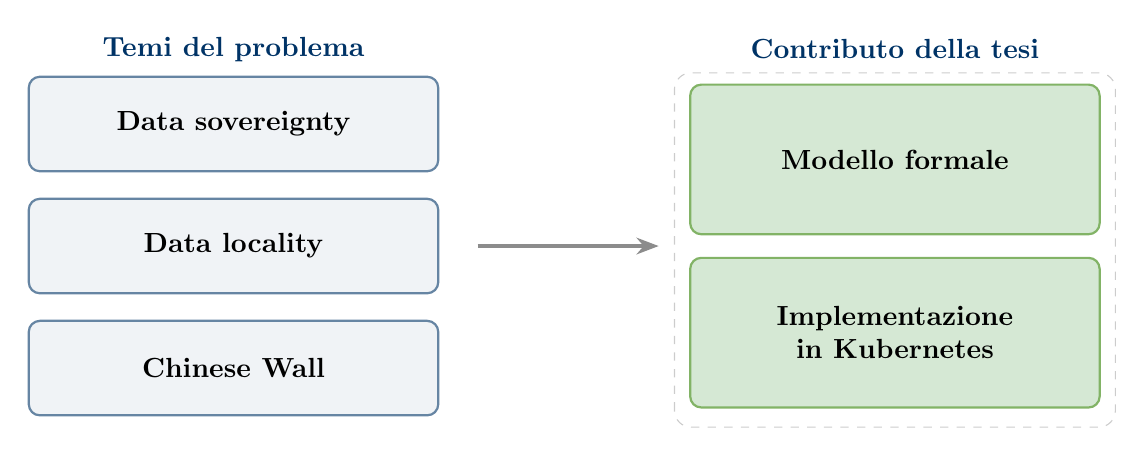
\begin{tikzpicture}[
  hd/.style={font=\normalsize\bfseries, text=unimi},
  th/.style={draw=unimi!60, fill=unimi!6, rounded corners=4pt, thick, align=center, minimum width=5.2cm, minimum height=1.2cm, inner sep=4pt},
  co/.style={draw=diogreenborder, fill=diogreen, rounded corners=4pt, thick, align=center, minimum width=5.2cm, minimum height=1.9cm, inner sep=4pt},
  ar/.style={-{Stealth[length=8pt]}, line width=1.4pt, black!45}]
  \node[hd] at (2.8,2.75) {Temi del problema};
  \node[hd] at (11.2,2.75) {Contributo della tesi};
  \node[th] (a) at (2.8,1.8) {\normalsize\bfseries Data sovereignty};
  \node[th] (b) at (2.8,0.25) {\normalsize\bfseries Data locality};
  \node[th] (c) at (2.8,-1.3) {\normalsize\bfseries Chinese Wall};
  \node[co] (m) at (11.2,1.35) {\normalsize\bfseries Modello formale};
  \node[co] (k) at (11.2,-0.85) {\normalsize\bfseries Implementazione \\ \normalsize\bfseries in Kubernetes};
  \draw[black!20, rounded corners=6pt, dashed] (8.4,-2.05) rectangle (14.0,2.45);
  \draw[ar] (5.9,0.25) -- (8.2,0.25);
\end{tikzpicture}
\end{center}

\note{Questo problema tocca tre ambiti di ricerca noti:
\begin{itemize}
\item la \textbf{data sovereignty}, da cui derivano determinati vincoli geografici;
\item la \textbf{data locality}, per portare il calcolo vicino ai dati, sia per risparmiare banda sia perché certi dati non si possono trasferire;
\item e infine il modello di \textbf{Chinese Wall}, per isolare i nodi dalle tracce che i task lasciano in memoria.
\end{itemize}
La tesi li riunisce in un unico meccanismo di scelta del nodo, con un modello formale che li traduce in politiche e un'implementazione concreta in Kubernetes.}
\end{frame}

% ===========================================================================
\begin{frame}{Il problema: dove eseguire il task?}
\begin{center}
\vspace{2mm}
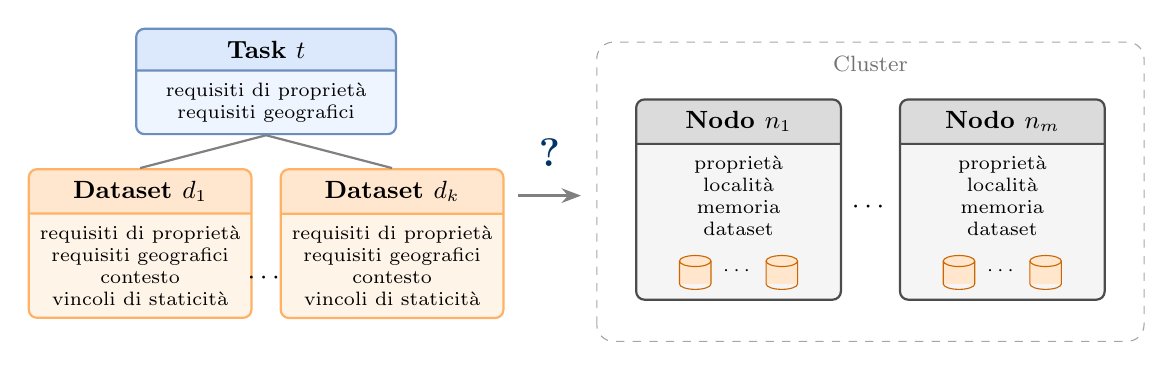
\begin{tikzpicture}[
  bx/.style={rectangle split, rectangle split parts=2, rectangle split part fill={gray!28,gray!8},
             rounded corners=3pt, draw=black!70, thick, align=center, font=\scriptsize, inner sep=4pt},
  tk/.style={bx, rectangle split part fill={dioblue!95,dioblue!45}, draw=dioblueborder, minimum width=3.3cm},
  dsb/.style={bx, rectangle split part fill={dioorange!95,dioorange!45}, draw=orange!60, minimum width=2.6cm},
  nd/.style={bx, minimum width=2.6cm},
  db/.pic={\fill[dioorange] (-0.2,-0.145) rectangle (0.2,0.145);
           \draw[orange!80!black] (-0.2,-0.145) -- (-0.2,0.145) (0.2,-0.145) -- (0.2,0.145) (-0.2,-0.145) arc (180:360:0.2 and 0.07);
           \draw[orange!80!black, fill=dioorange] (0,0.145) ellipse (0.2 and 0.07);}]
  % task e dataset
  \node[tk] (task) at (2.95,2.05) {\textbf{\small Task $t$}\nodepart{two}requisiti di proprietà\\requisiti geografici};
  \node[dsb, anchor=north] (d1) at (1.35,0.95) {\textbf{\small Dataset $d_1$}\nodepart{two}requisiti di proprietà\\requisiti geografici\\contesto\\vincoli di staticità};
  \node[dsb, anchor=north] (dk) at (4.55,0.95) {\textbf{\small Dataset $d_k$}\nodepart{two}requisiti di proprietà\\requisiti geografici\\contesto\\vincoli di staticità};
  \node at (2.95,-0.45) {$\cdots$};
  \draw[black!50, thick] (task.south) -- (d1.north);
  \draw[black!50, thick] (task.south) -- (dk.north);
  % freccia verso il cluster
  \draw[-{Stealth[length=7pt]}, very thick, black!50] (6.15,0.6) -- (6.95,0.6);
  \node[font=\Large\bfseries, text=unimi] at (6.55,1.15) {?};
  % cluster
  \draw[dashed, black!35, rounded corners=6pt] (7.15,-1.25) rectangle (14.1,2.55);
  \node[font=\footnotesize, text=black!55] at (10.625,2.28) {Cluster};
  \node[nd] (n1) at (8.95,0.55) {\textbf{\small Nodo $n_1$}\nodepart{two}proprietà\\località\\memoria\\dataset\\\rule{0pt}{0.62cm}};
  \node[nd] (nm) at (12.3,0.55) {\textbf{\small Nodo $n_m$}\nodepart{two}proprietà\\località\\memoria\\dataset\\\rule{0pt}{0.62cm}};
  \node at (10.625,0.45) {$\cdots$};
  \foreach \n in {n1,nm} {
    \pic at ($(\n.south)+(-0.55,0.36)$) {db};
    \pic at ($(\n.south)+(0.55,0.36)$) {db};
    \node[font=\scriptsize] at ($(\n.south)+(0,0.38)$) {$\cdots$};
  }
\end{tikzpicture}
\end{center}

\note{Ora guardiamo il problema più da vicino. Da una parte ci sono \textbf{i nodi}, ognuno con un livello per ogni proprietà, una località e i dataset che ospita, che possono comunque essere trasferiti altrove.

Dall'altra c'è un \textbf{task che richiede dei dataset}, e bisogna \textbf{scegliere} su quale nodo eseguirlo. Task e dataset dichiarano dei requisiti: un livello minimo per ogni proprietà e le aree geografiche in cui possono trovarsi. I dataset hanno inoltre un contesto, cioè l'ambito o l'organizzazione a cui appartengono, e possono essere statici, cioè non trasferibili.

Il problema \textbf{non è banale} perché questi vincoli arrivano da entità diverse, e il nodo scelto deve rispettarli tutti contemporaneamente.}
\end{frame}

% ===========================================================================
\begin{frame}{Il modello: prima si filtra, poi si sceglie}
\begin{center}
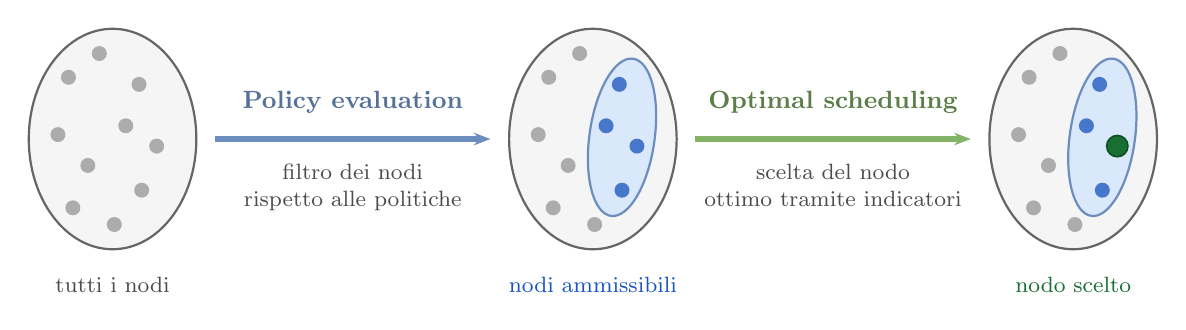
\begin{tikzpicture}[
  dot/.style={circle, fill=gray!65, inner sep=0pt, minimum size=0.19cm},
  bdot/.style={circle, fill=reqblue!80, inner sep=0pt, minimum size=0.19cm},
  ar/.style={-{Stealth[length=6pt]}, very thick, black!60},
  lb/.style={font=\footnotesize, text=black!70, align=center},
  ph/.style={font=\small\bfseries, align=center},
  ds/.style={font=\footnotesize, text=black!70, align=center}]
  \draw[thick, black!60, fill=gray!8] (0,0) ellipse (1.064 and 1.400);
  \node[dot] at (-0.560,0.784) {};
  \node[dot] at (-0.168,1.086) {};
  \node[dot] at (-0.694,0.056) {};
  \node[dot] at (-0.314,-0.336) {};
  \node[dot] at (-0.504,-0.874) {};
  \node[dot] at (0.022,-1.086) {};
  \node[dot] at (0.336,0.694) {};
  \node[dot] at (0.168,0.168) {};
  \node[dot] at (0.560,-0.090) {};
  \node[dot] at (0.370,-0.650) {};
  \draw[thick, black!60, fill=gray!8] (6.1,0) ellipse (1.064 and 1.400);
  \draw[thick, dioblueborder, fill=dioblue, rotate around={-8:(6.470,0.022)}] (6.470,0.022) ellipse (0.414 and 1.008);
  \node[dot] at (5.540,0.784) {};
  \node[dot] at (5.932,1.086) {};
  \node[dot] at (5.406,0.056) {};
  \node[dot] at (5.786,-0.336) {};
  \node[dot] at (5.596,-0.874) {};
  \node[dot] at (6.122,-1.086) {};
  \node[bdot] at (6.436,0.694) {};
  \node[bdot] at (6.268,0.168) {};
  \node[bdot] at (6.660,-0.090) {};
  \node[bdot] at (6.470,-0.650) {};
  \draw[thick, black!60, fill=gray!8] (12.2,0) ellipse (1.064 and 1.400);
  \draw[thick, dioblueborder, fill=dioblue, rotate around={-8:(12.570,0.022)}] (12.570,0.022) ellipse (0.414 and 1.008);
  \node[dot] at (11.640,0.784) {};
  \node[dot] at (12.032,1.086) {};
  \node[dot] at (11.506,0.056) {};
  \node[dot] at (11.886,-0.336) {};
  \node[dot] at (11.696,-0.874) {};
  \node[dot] at (12.222,-1.086) {};
  \node[bdot] at (12.536,0.694) {};
  \node[bdot] at (12.368,0.168) {};
  \node[circle, fill=okgreen!85!black, draw=okgreen!60!black, line width=0.6pt, inner sep=0pt, minimum size=0.27cm] at (12.760,-0.090) {};
  \node[bdot] at (12.570,-0.650) {};
  \draw[ar, dioblueborder, line width=2pt] (1.3,0) -- (4.8,0);
  \draw[ar, diogreenborder, line width=2pt] (7.4,0) -- (10.9,0);
  \node[ph, text=dioblueborder!80!black, anchor=south] at (3.05,0.2) {Policy evaluation};
  \node[ds, anchor=north] at (3.05,-0.2) {filtro dei nodi\\rispetto alle politiche};
  \node[ph, text=diogreenborder!70!black, anchor=south] at (9.15,0.2) {Optimal scheduling};
  \node[ds, anchor=north] at (9.15,-0.2) {scelta del nodo\\ottimo tramite indicatori};
  \node[lb] at (0,-1.85) {tutti i nodi};
  \node[lb] at (6.1,-1.85) {\textcolor{reqblue}{nodi ammissibili}};
  \node[lb] at (12.2,-1.85) {\textcolor{okgreen!85!black}{nodo scelto}};
\end{tikzpicture}
\end{center}

\note{Per scegliere il nodo su cui eseguire il task, il modello segue due fasi. Nella prima, si parte da tutti i nodi del cluster per poi \textbf{filtrarli} rispetto ad un \textbf{insieme di politiche} che devono rispettare per poter rimanere nell'insieme dei nodi ammissibili. 

Poi, nella seconda, ad ogni nodo ammissibile viene \textbf{assegnato un punteggio} sulla base di un insieme di indicatori, che ne valutano l'ottimalità secondo determinate metriche. I punteggi vengono infine combinati selezionando il nodo con il punteggio più alto.

Ora vediamo le politiche in questione, partendo da quelle statiche.}
\end{frame}

% ===========================================================================
\begin{frame}{Politiche statiche}
\begin{center}
\vspace{-5mm}
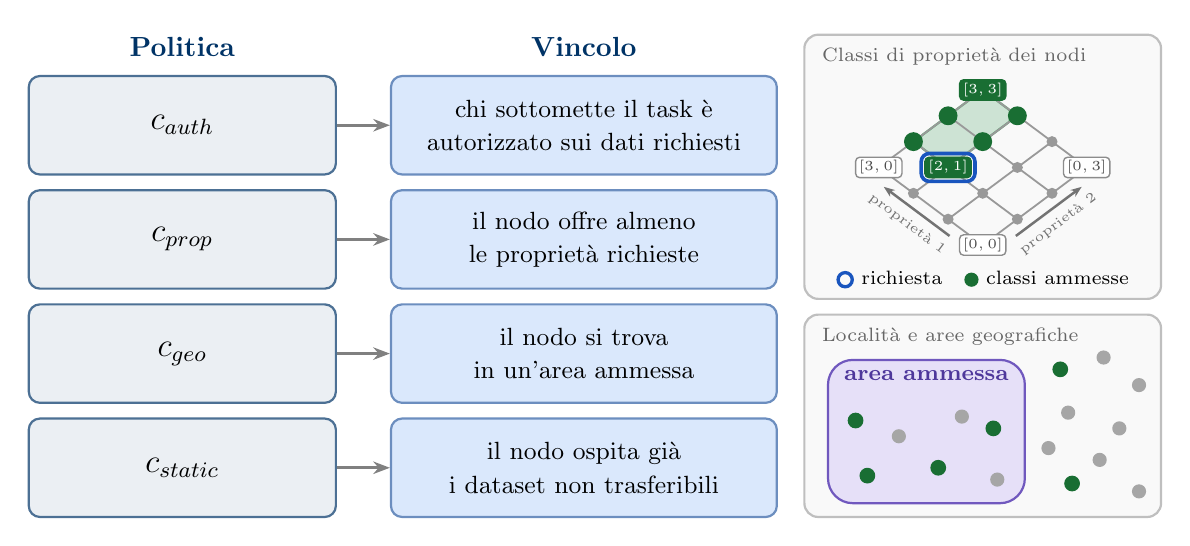
\begin{tikzpicture}[
  hd/.style={font=\normalsize\bfseries, text=unimi},
  pol/.style={rounded corners=4pt, thick, draw=unimi!70, fill=unimi!8, minimum width=3.9cm, minimum height=1.25cm, inner sep=2pt, align=center},
  vin/.style={rounded corners=4pt, thick, draw=dioblueborder, fill=dioblue, minimum width=4.9cm, minimum height=1.25cm, inner sep=2pt, align=center},
  pan/.style={rounded corners=5pt, thick, draw=black!25, fill=gray!5},
  ttl/.style={font=\scriptsize, text=black!60, anchor=north west},
  ar/.style={-{Stealth[length=6pt]}, very thick, black!50}]
  \node[hd] at (1.95,3.1) {Politica};
  \node[hd] at (7.05,3.1) {Vincolo};
  \node[pol] (p0) at (1.95,2.1) {\large $c_{auth}$};
  \node[vin] (v0) at (7.05,2.1) {{\small chi sottomette il task è}\\{\small autorizzato sui dati richiesti}};
  \draw[ar] (p0.east) -- (v0.west);
  \node[pol] (p1) at (1.95,0.65) {\large $c_{prop}$};
  \node[vin] (v1) at (7.05,0.65) {{\small il nodo offre almeno}\\{\small le proprietà richieste}};
  \draw[ar] (p1.east) -- (v1.west);
  \node[pol] (p2) at (1.95,-0.8) {\large $c_{geo}$};
  \node[vin] (v2) at (7.05,-0.8) {{\small il nodo si trova}\\{\small in un'area ammessa}};
  \draw[ar] (p2.east) -- (v2.west);
  \node[pol] (p3) at (1.95,-2.25) {\large $c_{static}$};
  \node[vin] (v3) at (7.05,-2.25) {{\small il nodo ospita già}\\{\small i dataset non trasferibili}};
  \draw[ar] (p3.east) -- (v3.west);
  \draw[pan] (9.85,-0.105) rectangle (14.38,3.25);
  \draw[pan] (9.85,-2.875) rectangle (14.38,-0.305);
  \node[ttl] at (9.95,3.2) {Classi di proprietà dei nodi};
  \node[ttl] at (9.95,-0.355) {Località e aree geografiche};
  \fill[okgreen!22, draw=okgreen!70, thick, rounded corners=4pt] (11.675,1.564) -- (11.235,1.892) -- (12.115,2.548) -- (12.555,2.220) -- cycle;
  \draw[black!40, line width=0.65pt] (12.115,0.579) -- (11.675,0.907);
  \draw[black!40, line width=0.65pt] (12.115,0.579) -- (12.555,0.907);
  \draw[black!40, line width=0.65pt] (12.555,0.907) -- (12.115,1.236);
  \draw[black!40, line width=0.65pt] (12.555,0.907) -- (12.995,1.236);
  \draw[black!40, line width=0.65pt] (12.995,1.236) -- (12.555,1.564);
  \draw[black!40, line width=0.65pt] (12.995,1.236) -- (13.435,1.564);
  \draw[black!40, line width=0.65pt] (13.435,1.564) -- (12.995,1.892);
  \draw[black!40, line width=0.65pt] (11.675,0.907) -- (11.235,1.236);
  \draw[black!40, line width=0.65pt] (11.675,0.907) -- (12.115,1.236);
  \draw[black!40, line width=0.65pt] (12.115,1.236) -- (11.675,1.564);
  \draw[black!40, line width=0.65pt] (12.115,1.236) -- (12.555,1.564);
  \draw[black!40, line width=0.65pt] (12.555,1.564) -- (12.115,1.892);
  \draw[black!40, line width=0.65pt] (12.555,1.564) -- (12.995,1.892);
  \draw[black!40, line width=0.65pt] (12.995,1.892) -- (12.555,2.220);
  \draw[black!40, line width=0.65pt] (11.235,1.236) -- (10.795,1.564);
  \draw[black!40, line width=0.65pt] (11.235,1.236) -- (11.675,1.564);
  \draw[black!40, line width=0.65pt] (11.675,1.564) -- (11.235,1.892);
  \draw[black!40, line width=0.65pt] (11.675,1.564) -- (12.115,1.892);
  \draw[black!40, line width=0.65pt] (12.115,1.892) -- (11.675,2.220);
  \draw[black!40, line width=0.65pt] (12.115,1.892) -- (12.555,2.220);
  \draw[black!40, line width=0.65pt] (12.555,2.220) -- (12.115,2.548);
  \draw[black!40, line width=0.65pt] (10.795,1.564) -- (11.235,1.892);
  \draw[black!40, line width=0.65pt] (11.235,1.892) -- (11.675,2.220);
  \draw[black!40, line width=0.65pt] (11.675,2.220) -- (12.115,2.548);
  \node[fill=white, draw=black!45, text=black!70, rounded corners=1.5pt, inner sep=1.2pt, font=\tiny, line width=0.5pt] at (12.115,0.579) {$[0,0]$};
  \fill[black!40] (12.555,0.907) circle (0.07);
  \fill[black!40] (12.995,1.236) circle (0.07);
  \node[fill=white, draw=black!45, text=black!70, rounded corners=1.5pt, inner sep=1.2pt, font=\tiny, line width=0.5pt] at (13.435,1.564) {$[0,3]$};
  \fill[black!40] (11.675,0.907) circle (0.07);
  \fill[black!40] (12.115,1.236) circle (0.07);
  \fill[black!40] (12.555,1.564) circle (0.07);
  \fill[black!40] (12.995,1.892) circle (0.07);
  \fill[black!40] (11.235,1.236) circle (0.07);
  \fill[okgreen!85!black] (12.115,1.892) circle (0.12);
  \fill[okgreen!85!black] (12.555,2.220) circle (0.12);
  \node[fill=white, draw=black!45, text=black!70, rounded corners=1.5pt, inner sep=1.2pt, font=\tiny, line width=0.5pt] at (10.795,1.564) {$[3,0]$};
  \fill[okgreen!85!black] (11.235,1.892) circle (0.12);
  \fill[okgreen!85!black] (11.675,2.220) circle (0.12);
  \node[fill=okgreen!85!black, draw=okgreen!85!black, text=white, rounded corners=1.5pt, inner sep=1.2pt, font=\tiny, line width=0.5pt] at (12.115,2.548) {$[3,3]$};
  \node[fill=okgreen!85!black, draw=okgreen!85!black, text=white, rounded corners=1.5pt, inner sep=1.2pt, font=\tiny, line width=0.5pt] (req) at (11.675,1.564) {$[2,1]$};
  \draw[reqblue, line width=1.3pt, rounded corners=3pt] ([shift={(-1.1pt,-1.1pt)}]req.south west) rectangle ([shift={(1.1pt,1.1pt)}]req.north east);
  \draw[-{Stealth[length=4pt]}, black!55, line width=0.9pt] (11.694,0.694) -- (10.858,1.318);
  \node[font=\tiny, text=black!55, rotate=-36.75, inner sep=0pt] at (11.156,0.846) {proprietà 1};
  \draw[-{Stealth[length=4pt]}, black!55, line width=0.9pt] (12.536,0.694) -- (13.372,1.318);
  \node[font=\tiny, text=black!55, rotate=36.75, inner sep=0pt] at (13.074,0.846) {proprietà 2};
  \node[font=\scriptsize, anchor=base] at (12.115,0.075) {\tikz[baseline=-0.6ex]\draw[reqblue, line width=1.2pt] (0,0) circle (0.09);\ richiesta\quad \tikz[baseline=-0.6ex]\fill[okgreen!85!black] (0,0) circle (0.09);\ classi ammesse};
  \draw[rounded corners=9pt, thick, draw=areaborder, fill=areafill] (10.15,-2.700) rectangle (12.65,-0.880);
  \node[font=\footnotesize\bfseries, text=areatext, anchor=north, inner sep=1pt] at (11.4,-0.970) {area ammessa};
  \fill[black!35] (11.05,-1.85) circle (0.09);
  \fill[black!35] (11.85,-1.6) circle (0.09);
  \fill[black!35] (12.3,-2.4) circle (0.09);
  \fill[black!35] (13.65,-0.85) circle (0.09);
  \fill[black!35] (14.1,-1.2) circle (0.09);
  \fill[black!35] (13.2,-1.55) circle (0.09);
  \fill[black!35] (12.95,-2.0) circle (0.09);
  \fill[black!35] (13.6,-2.15) circle (0.09);
  \fill[black!35] (14.1,-2.55) circle (0.09);
  \fill[okgreen!85!black] (10.5,-1.65) circle (0.1);
  \fill[okgreen!85!black] (11.55,-2.25) circle (0.1);
  \fill[okgreen!85!black] (12.25,-1.75) circle (0.1);
  \fill[okgreen!85!black] (13.1,-1.0) circle (0.1);
  \fill[black!35] (13.85,-1.75) circle (0.09);
  \fill[okgreen!85!black] (13.25,-2.45) circle (0.1);
  \fill[okgreen!85!black] (10.65,-2.35) circle (0.1);
\end{tikzpicture}
\end{center}

\note{Le politiche statiche, cioè che non dipendono dallo stato del cluster, sono quattro. La prima, $c_{auth}$, richiede che chi sottomette il task sia \textbf{autorizzato} sui dati che richiede, altrimenti il task viene rifiutato subito.

Poi $c_{prop}$ richiede che il nodo candidato abbia \textbf{almeno il livello richiesto} su ogni proprietà. I livelli di un nodo formano la sua classe di proprietà, mentre il task, insieme ai suoi dataset, richiede una classe minima; ordinando le classi si ottiene una vista a reticolo come in figura, e il nodo è ammesso per quel task solo se la sua classe domina quella richiesta.

Infine, $c_{geo}$ richiede che il nodo candidato si trovi in un'\textbf{area geografica ammessa} sia dal task sia dai suoi dataset, e $c_{static}$ che ospiti già i dataset \textbf{non trasferibili} richiesti.}
\end{frame}

% ===========================================================================
\begin{frame}{La politica dinamica: Chinese Wall sui nodi}
\begin{columns}[T]
\column{0.46\textwidth}
\centering
\textbf{\color{unimi}Politica $c_{wall}$}\\[3mm]
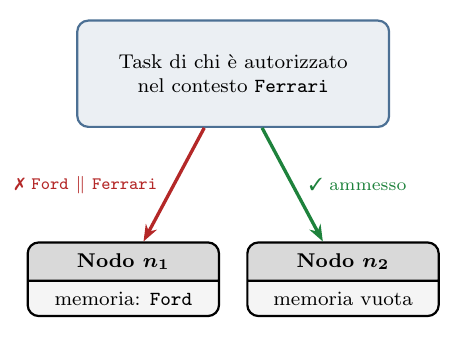
\begin{tikzpicture}[scale=0.9, transform shape,
    nd/.style={rectangle split, rectangle split parts=2, rectangle split part fill={gray!30,gray!8}, rounded corners=4pt, draw=black, thick, minimum width=2.7cm, align=center, font=\footnotesize, inner sep=4pt, minimum height=1.5cm},
    tk/.style={rectangle, rounded corners=4pt, draw=unimi!70, thick, fill=unimi!8, align=center, font=\footnotesize, minimum width=4.4cm, minimum height=1.5cm},
    lab/.style={font=\scriptsize, align=center}]
  \useasboundingbox (-2.9,-0.55) rectangle (2.9,3.55);
  \node[tk] (t) at (0,2.9) {Task di chi è autorizzato\\nel contesto \texttt{Ferrari}};
  \node[nd] (n1) at (-1.55,0) {\textbf{Nodo $\boldsymbol{n_1}$}\nodepart{two}memoria: \texttt{Ford}};
  \node[nd] (n2) at (1.55,0) {\textbf{Nodo $\boldsymbol{n_2}$}\nodepart{two}memoria vuota};
  \draw[-{Stealth[length=6pt]}, very thick, kored] (t) -- node[lab, left=1mm, text=kored, align=right] {\ko\ \texttt{Ford} $\parallel$ \texttt{Ferrari}} (n1);
  \draw[-{Stealth[length=6pt]}, very thick, okgreen] (t) -- node[lab, right=1mm, text=okgreen] {\ok\ ammesso} (n2);
\end{tikzpicture}
\column{0.50\textwidth}
\centering
\textbf{\color{unimi}Sanificazione}\\[3mm]
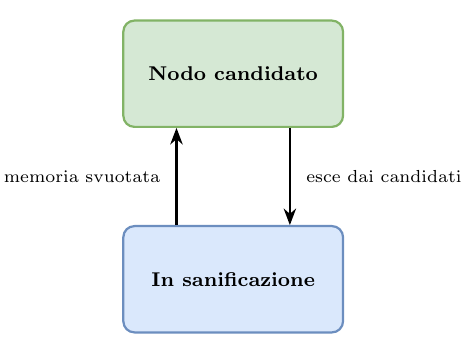
\begin{tikzpicture}[scale=0.9, transform shape,
    st/.style={rounded corners=4pt, thick, align=center, font=\footnotesize, minimum width=3.1cm, minimum height=1.5cm},
    ar/.style={-{Stealth[length=6pt]}, thick},
    lab/.style={font=\scriptsize}]
  \useasboundingbox (-2.9,-0.55) rectangle (2.9,3.55);
  \node[st, draw=diogreenborder, fill=diogreen] (c) at (0,2.9) {\textbf{Nodo candidato}};
  \node[st, draw=dioblueborder, fill=dioblue] (s) at (0,0) {\textbf{In sanificazione}};
  \draw[ar] ([xshift=0.8cm]c.south) -- node[right=1mm, lab] {esce dai candidati} ([xshift=0.8cm]s.north);
  \draw[ar] ([xshift=-0.8cm]s.north) -- node[left=1mm, lab] {memoria svuotata} ([xshift=-0.8cm]c.south);
\end{tikzpicture}
\end{columns}
\note{Arriviamo alla politica dinamica, che riprende il modello di \textbf{Chinese Wall} per i conflitti di interesse, applicato ai nodi. 

Ogni esecuzione può lasciare sul nodo \textbf{tracce dei dati elaborati} che un task successivo potrebbe leggere. Per questo ogni nodo mantiene una \textbf{memoria dei contesti} dei dati che ha trattato, e $c_{wall}$ lo esclude se chi sottomette il task è autorizzato su un contesto in conflitto con uno di quelli in memoria. Nell'esempio il primo nodo ha elaborato dati Ford, in conflitto con il contesto Ferrari del task, e viene escluso, mentre il secondo resta disponibile.

Col tempo, però, la memoria si riempirebbe e i nodi finirebbero esclusi quasi per tutti. Per evitare questa \textbf{starvation}, ogni nodo viene periodicamente sanificato e la sua memoria svuotata.}
\end{frame}

% ===========================================================================
\begin{frame}{Gli indicatori: scegliere tra i nodi ammissibili}
\begin{center}
\vspace{2mm}
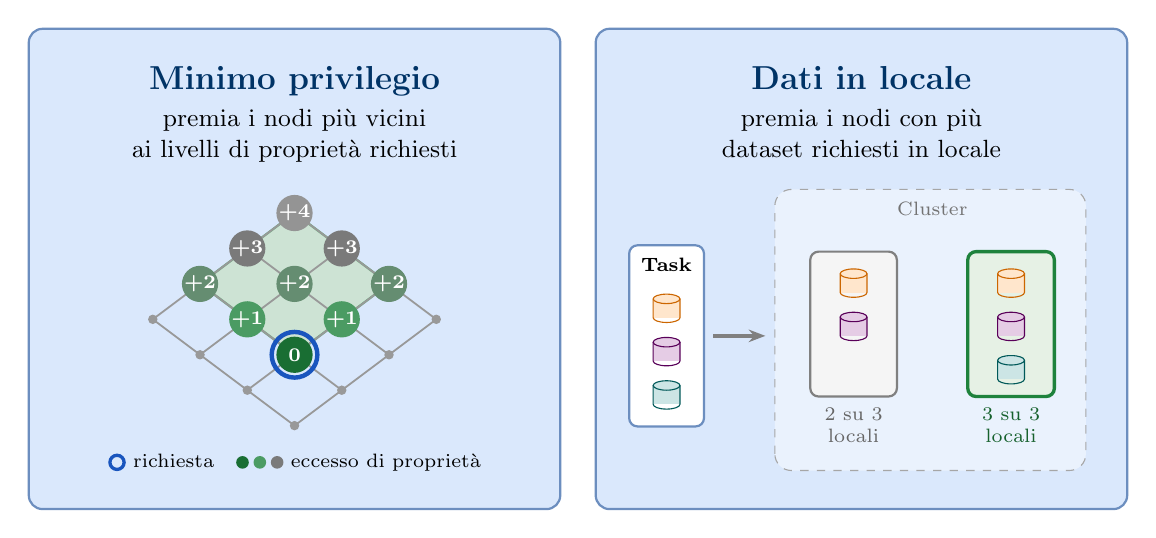
\begin{tikzpicture}[
  ib/.style={rounded corners=5pt, draw=dioblueborder, fill=dioblue, thick, minimum width=6.75cm, minimum height=6.1cm},
  pics/dbc0/.style={code={\fill[dioorange] (-0.17,-0.12) rectangle (0.17,0.12); \draw[orange!80!black] (-0.17,-0.12) -- (-0.17,0.12) (0.17,-0.12) -- (0.17,0.12) (-0.17,-0.12) arc (180:360:0.17 and 0.06); \draw[orange!80!black, fill=dioorange] (0,0.12) ellipse (0.17 and 0.06);}},
  pics/dbc1/.style={code={\fill[violet!20] (-0.17,-0.12) rectangle (0.17,0.12); \draw[violet!70!black] (-0.17,-0.12) -- (-0.17,0.12) (0.17,-0.12) -- (0.17,0.12) (-0.17,-0.12) arc (180:360:0.17 and 0.06); \draw[violet!70!black, fill=violet!20] (0,0.12) ellipse (0.17 and 0.06);}},
  pics/dbc2/.style={code={\fill[teal!20] (-0.17,-0.12) rectangle (0.17,0.12); \draw[teal!70!black] (-0.17,-0.12) -- (-0.17,0.12) (0.17,-0.12) -- (0.17,0.12) (-0.17,-0.12) arc (180:360:0.17 and 0.06); \draw[teal!70!black, fill=teal!20] (0,0.12) ellipse (0.17 and 0.06);}}]
  \node[ib] (a) at (-3.6,0) {};
  \node[ib] (b) at (3.6,0) {};
  \node[font=\large\bfseries, text=unimi, anchor=north] at (-3.6,2.70) {Minimo privilegio};
  \node[font=\small, align=center, anchor=north] at (-3.6,2.15) {premia i nodi più vicini\\ai livelli di proprietà richiesti};
  \node[font=\large\bfseries, text=unimi, anchor=north] at (3.6,2.70) {Dati in locale};
  \node[font=\small, align=center, anchor=north] at (3.6,2.15) {premia i nodi con più\\dataset richiesti in locale};
  \fill[okgreen!22, draw=okgreen!70, thick, rounded corners=5pt] (-3.600,-1.090) -- (-2.400,-0.190) -- (-3.600,0.710) -- (-4.800,-0.190) -- cycle;
  \draw[black!40, line width=0.65pt] (-3.600,-1.990) -- (-3.000,-1.540);
  \draw[black!40, line width=0.65pt] (-3.600,-1.990) -- (-4.200,-1.540);
  \draw[black!40, line width=0.65pt] (-4.200,-1.540) -- (-3.600,-1.090);
  \draw[black!40, line width=0.65pt] (-4.200,-1.540) -- (-4.800,-1.090);
  \draw[black!40, line width=0.65pt] (-4.800,-1.090) -- (-4.200,-0.640);
  \draw[black!40, line width=0.65pt] (-4.800,-1.090) -- (-5.400,-0.640);
  \draw[black!40, line width=0.65pt] (-5.400,-0.640) -- (-4.800,-0.190);
  \draw[black!40, line width=0.65pt] (-3.000,-1.540) -- (-2.400,-1.090);
  \draw[black!40, line width=0.65pt] (-3.000,-1.540) -- (-3.600,-1.090);
  \draw[black!40, line width=0.65pt] (-3.600,-1.090) -- (-3.000,-0.640);
  \draw[black!40, line width=0.65pt] (-3.600,-1.090) -- (-4.200,-0.640);
  \draw[black!40, line width=0.65pt] (-4.200,-0.640) -- (-3.600,-0.190);
  \draw[black!40, line width=0.65pt] (-4.200,-0.640) -- (-4.800,-0.190);
  \draw[black!40, line width=0.65pt] (-4.800,-0.190) -- (-4.200,0.260);
  \draw[black!40, line width=0.65pt] (-2.400,-1.090) -- (-1.800,-0.640);
  \draw[black!40, line width=0.65pt] (-2.400,-1.090) -- (-3.000,-0.640);
  \draw[black!40, line width=0.65pt] (-3.000,-0.640) -- (-2.400,-0.190);
  \draw[black!40, line width=0.65pt] (-3.000,-0.640) -- (-3.600,-0.190);
  \draw[black!40, line width=0.65pt] (-3.600,-0.190) -- (-3.000,0.260);
  \draw[black!40, line width=0.65pt] (-3.600,-0.190) -- (-4.200,0.260);
  \draw[black!40, line width=0.65pt] (-4.200,0.260) -- (-3.600,0.710);
  \draw[black!40, line width=0.65pt] (-1.800,-0.640) -- (-2.400,-0.190);
  \draw[black!40, line width=0.65pt] (-2.400,-0.190) -- (-3.000,0.260);
  \draw[black!40, line width=0.65pt] (-3.000,0.260) -- (-3.600,0.710);
  \fill[black!40] (-3.600,-1.990) circle (0.06);
  \fill[black!40] (-4.200,-1.540) circle (0.06);
  \fill[black!40] (-4.800,-1.090) circle (0.06);
  \fill[black!40] (-5.400,-0.640) circle (0.06);
  \fill[black!40] (-3.000,-1.540) circle (0.06);
  \node[circle, fill=okgreen!85!black, inner sep=0pt, minimum size=0.46cm, font=\scriptsize\bfseries, text=white] at (-3.600,-1.090) {0};
  \node[circle, fill=okgreen!80, inner sep=0pt, minimum size=0.46cm, font=\scriptsize\bfseries, text=white] at (-4.200,-0.640) {+1};
  \node[circle, fill=okgreen!45!gray!90, inner sep=0pt, minimum size=0.46cm, font=\scriptsize\bfseries, text=white] at (-4.800,-0.190) {+2};
  \fill[black!40] (-2.400,-1.090) circle (0.06);
  \node[circle, fill=okgreen!80, inner sep=0pt, minimum size=0.46cm, font=\scriptsize\bfseries, text=white] at (-3.000,-0.640) {+1};
  \node[circle, fill=okgreen!45!gray!90, inner sep=0pt, minimum size=0.46cm, font=\scriptsize\bfseries, text=white] at (-3.600,-0.190) {+2};
  \node[circle, fill=black!52, inner sep=0pt, minimum size=0.46cm, font=\scriptsize\bfseries, text=white] at (-4.200,0.260) {+3};
  \fill[black!40] (-1.800,-0.640) circle (0.06);
  \node[circle, fill=okgreen!45!gray!90, inner sep=0pt, minimum size=0.46cm, font=\scriptsize\bfseries, text=white] at (-2.400,-0.190) {+2};
  \node[circle, fill=black!52, inner sep=0pt, minimum size=0.46cm, font=\scriptsize\bfseries, text=white] at (-3.000,0.260) {+3};
  \node[circle, fill=black!42, inner sep=0pt, minimum size=0.46cm, font=\scriptsize\bfseries, text=white] at (-3.600,0.710) {+4};
  \draw[reqblue, line width=1.6pt] (-3.600,-1.090) circle (0.29);
  \node[font=\scriptsize, anchor=base] at (-3.600,-2.520) {\tikz[baseline=-0.6ex]\draw[reqblue, line width=1.2pt] (0,0) circle (0.09);\ richiesta\quad \tikz[baseline=-0.6ex]{\fill[okgreen!85!black] (0,0) circle (0.08); \fill[okgreen!80] (0.22,0) circle (0.08); \fill[black!52] (0.44,0) circle (0.08);}\ eccesso di proprietà};
  \draw[rounded corners=3pt, thick, draw=dioblueborder, fill=white] (0.65,-2.00) rectangle (1.60,0.30);
  \node[font=\scriptsize\bfseries] at (1.125,0.05) {Task};
  \pic at (1.125,-0.500) {dbc0};
  \pic at (1.125,-1.050) {dbc1};
  \pic at (1.125,-1.600) {dbc2};
  \draw[-{Stealth[length=6pt]}, very thick, black!50] (1.72,-0.85) -- (2.38,-0.85);
  \draw[rounded corners=6pt, dashed, draw=black!35, fill=white, fill opacity=0.45] (2.5,-2.56) rectangle (6.45,1.01);
  \node[font=\scriptsize, text=black!55] at (4.5,0.76) {Cluster};
  \draw[rounded corners=3pt, thick, draw=black!50, fill=gray!8] (2.95,-1.62) rectangle (4.05,0.22);
  \draw[rounded corners=3pt, very thick, draw=okgreen, fill=diogreen!60] (4.95,-1.62) rectangle (6.05,0.22);
  \node[font=\scriptsize, text=black!60, align=center, inner sep=0pt] at (3.5,-1.98) {2 su 3\\locali};
  \node[font=\scriptsize, text=okgreen!75!black, align=center, inner sep=0pt] at (5.5,-1.98) {3 su 3\\locali};
  \pic at (3.500,-0.180) {dbc0};
  \pic at (3.500,-0.730) {dbc1};
  \pic at (5.500,-0.180) {dbc0};
  \pic at (5.500,-0.730) {dbc1};
  \pic at (5.500,-1.280) {dbc2};
\end{tikzpicture}
\end{center}
\note{Tra i nodi ammissibili, si sceglie quello ottimo con due indicatori. Il primo segue il principio del \textbf{minimo privilegio}, premiando i nodi che superano di meno i livelli richiesti, così da non occupare risorse più preziose del necessario.

Il secondo, invece, premia i nodi che hanno \textbf{più dataset richiesti in locale} per ridurre i trasferimenti e la banda consumata. La somma pesata dei due punteggi andrà a decidere il nodo da assegnare al task.

A questo punto il modello è completo.}
\end{frame}

% ===========================================================================
\begin{frame}{Implementazione in Kubernetes}
\centering
\vfill
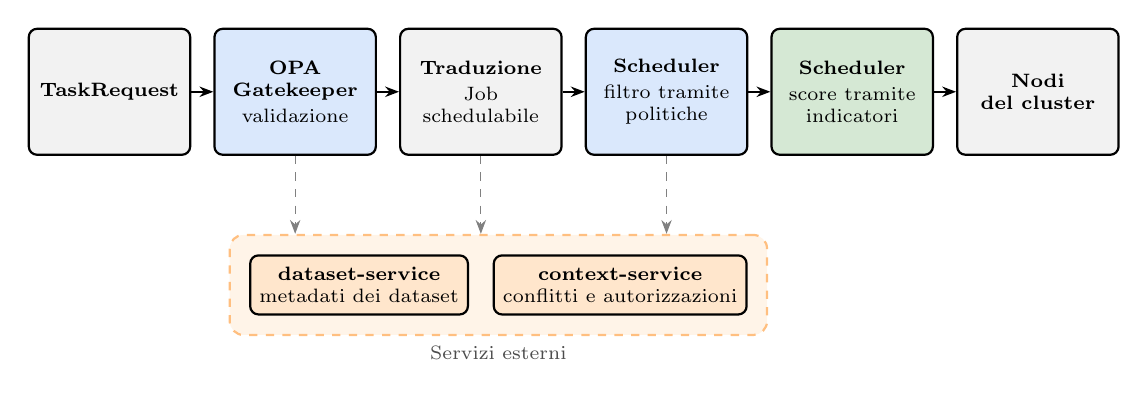
\begin{tikzpicture}[
    node distance=0.28cm,
    bx/.style={rectangle, rounded corners=3pt, draw=black, thick, minimum width=2.05cm, minimum height=1.6cm, align=center, font=\scriptsize, inner sep=3pt},
    sv/.style={rectangle, rounded corners=3pt, draw=black, thick, minimum width=2.5cm, minimum height=0.75cm, align=center, font=\scriptsize, fill=dioorange},
    ar/.style={-{Stealth[length=5pt]}, thick},
    da/.style={-{Stealth[length=5pt]}, dashed, gray}]
  \node[bx, fill=gray!10] (req) {\textbf{TaskRequest}};
  \node[bx, fill=dioblue, right=of req] (gk) {\textbf{OPA}\\\textbf{Gatekeeper}\\[0.5mm]validazione};
  \node[bx, fill=gray!10, right=of gk] (ctrl) {\textbf{Traduzione}\\[0.5mm]Job\\schedulabile};
  \node[bx, fill=dioblue, right=of ctrl] (sch) {\textbf{Scheduler}\\[0.5mm]filtro tramite\\politiche};
  \node[bx, fill=diogreen, right=of sch] (sc) {\textbf{Scheduler}\\[0.5mm]score tramite\\indicatori};
  \node[bx, fill=gray!10, right=of sc] (nodes) {\textbf{Nodi}\\\textbf{del cluster}};
  \draw[ar] (req) -- (gk); \draw[ar] (gk) -- (ctrl); \draw[ar] (ctrl) -- (sch); \draw[ar] (sch) -- (sc); \draw[ar] (sc) -- (nodes);
  \coordinate (mid) at ($(gk.south)!0.5!(sch.south)$);
  \node[sv, anchor=north east, xshift=-0.15cm] at ($(mid)+(0,-1.25)$) (ds) {\textbf{dataset-service}\\metadati dei dataset};
  \node[sv, anchor=north west, xshift=0.15cm] at ($(mid)+(0,-1.25)$) (cs) {\textbf{context-service}\\conflitti e autorizzazioni};
  \begin{scope}[on background layer]
    \node[draw=orange!50, dashed, thick, rounded corners=5pt, fill=dioorange!45, fit=(ds)(cs), inner sep=7pt,
          label={[font=\scriptsize, text=black!70]below:Servizi esterni}] (ext) {};
  \end{scope}
  \draw[da] (gk.south) -- (gk.south |- ext.north);
  \draw[da] (ctrl.south) -- (ctrl.south |- ext.north);
  \draw[da] (sch.south) -- (sch.south |- ext.north);
\end{tikzpicture}
\vfill

\note{Per l'implementazione ho sfruttato i \textbf{meccanismi di estensione} che offre Kubernetes, sviluppando una pipeline che segue le due fasi del modello.

Il task arriva come \textbf{risorsa Kubernetes}, viene validato da un controller di ammissione, OPA Gatekeeper, e poi tradotto in un Job \textbf{schedulabile}. Lo scheduler nativo esteso \textbf{filtra} quindi i nodi ammissibili tramite le politiche, scegliendo infine quello con il \textbf{punteggio migliore} rispetto agli indicatori.

Inoltre, lungo il percorso vengono interrogati due servizi esterni, uno per i metadati dei dataset e uno per conflitti e autorizzazioni.}
\end{frame}

% ===========================================================================
\begin{frame}{Valutazione: disponibilità dei nodi e latenza dei task}
\vspace{3mm}
\begin{columns}[c]
\column{0.49\textwidth}
\centering
\includegraphics[width=0.92\linewidth]{immagini/val_sanificazione/sanitize_disponibilita.jpg}\\
{\scriptsize Tempo in cui un nodo è fuori dai candidati}
\column{0.49\textwidth}
\centering
\includegraphics[width=0.92\linewidth]{immagini/val_sanificazione/sanitize_latenza.jpg}\\
{\scriptsize Latenza media di scheduling di un task}
\end{columns}

\note{Nella valutazione mi sono concentrato soprattutto sulla \textbf{componente dinamica} del modello, facendo variare ogni quanto i nodi vengono sanificati.

Ne emerge un \textbf{compromesso} tra la disponibilità dei nodi e la latenza di scheduling dei task. Infatti, sanificare \textbf{spesso} toglie i nodi dai candidati più a lungo, come si vede nel grafico a sinistra, mentre sanificare di \textbf{rado} può lasciare i task bloccati a lungo a causa delle tracce in conflitto sui nodi, come mostra la latenza a destra.}
\end{frame}

% ===========================================================================
\begin{frame}{Conclusioni e sviluppi futuri}
\vspace{4mm}
\begin{columns}[T]
\column{0.47\textwidth}
{\large\bfseries\color{unimi} Conclusioni}\\[3mm]
\begin{itemize}\setlength{\itemsep}{4mm}
\item Modello formale di scheduling guidato da politiche
\item Prototipo che lo realizza in Kubernetes
\end{itemize}
\column{0.47\textwidth}
{\large\bfseries\color{unimi} Sviluppi futuri}\\[3mm]
\begin{itemize}\setlength{\itemsep}{4mm}
\item Task con semantica propria e dati reali
\item Strategie ottimizzate di sanificazione
\item Estensione multi-cluster
\end{itemize}
\end{columns}

\note{Per concludere, la tesi propone un \textbf{modello formale} di scheduling guidato da politiche, che rispetta i vincoli di protezione dei dati, e un \textbf{prototipo} in Kubernetes che lo realizza.

Come sviluppi futuri, il primo è usare task e dati \textbf{reali}, dato che per ora il prototipo li simula a livello logico. Il secondo è adottare strategie di sanificazione \textbf{ottimizzate} per migliorare il compromesso analizzato. E per finire, estendere il sistema in ambiente \textbf{multi-cluster}.}
\end{frame}

% ===========================================================================
\begin{frame}[plain, noframenumbering]
\centering
\vspace*{\fill}

{\color{unimi}\fontsize{28}{34}\selectfont\bfseries Grazie per l'attenzione}

\vspace{4mm}

{\color{unimi!45}\rule{0.45\textwidth}{0.8pt}}

\vspace{4mm}

{\large Luca Milanesi}

\vspace{2mm}

{\normalsize Università degli Studi di Milano}

\vspace*{\fill}

\note{Vi ringrazio per l'attenzione, sono a disposizione per eventuali domande.}
\end{frame}

\newcounter{ultimaslide}
\setcounter{ultimaslide}{\value{framenumber}}

\ifdefined\CONRISERVA
% ===========================================================================
%  SLIDE DI RISERVA (per le domande)
% ===========================================================================
\setbeamertemplate{footline}{}
\begin{frame}{Riserva: formalizzazione del problema}
\vspace{-2mm}\begin{center}
{\small
\renewcommand{\arraystretch}{1.15}
\begin{tabular}{@{}r@{\hspace{5mm}}c@{\hspace{7mm}}c@{\hspace{7mm}}c@{\hspace{7mm}}c@{}}
{\color{unimi}\bfseries Insiemi principali} & $\mathcal{N}$ nodi & $\mathcal{D}$ dataset & $\mathcal{T}$ task & $\mathcal{I}$ issuer \\
{\color{unimi}\bfseries Funzioni base} & $iss : \mathcal{T} \rightarrow \mathcal{I}$ & $req : \mathcal{T} \rightarrow 2^{\mathcal{D}}$ & $\lambda : \mathcal{D} \rightarrow 2^{\mathcal{N}}$ & \\[-2.2mm]
 & {\scriptsize\color{black!60} issuer del task} & {\scriptsize\color{black!60} dataset richiesti} & {\scriptsize\color{black!60} nodi che lo ospitano} & \\
\end{tabular}\par}
\vspace{2mm}
\fcolorbox{unimi!40}{unimi!4}{\begin{minipage}{0.7\textwidth}\centering
$f(t) =
\begin{cases}
\arg\max\limits_{n \in \mathcal{F_C}(t)} \mathcal{S}_\Phi(n,t) & \text{se } \mathcal{F_C}(t) \neq \emptyset \\[2mm]
\bot & \text{se } \mathcal{F_C}(t) = \emptyset
\end{cases}$
\end{minipage}}
\end{center}
\vspace{0mm}
\begin{columns}[t]
\column{0.47\textwidth}
\centering
\textbf{\color{unimi}Policy evaluation}\\[1mm]
{\small Nodi ammissibili per il task:\\[1mm]
$\mathcal{F_C}(t) = \{\, n \in \mathcal{N} \mid n \models_t \mathcal{C} \,\}$\\[1mm]
$\mathcal{C} = \underbrace{\mathcal{C_A}}_{\text{task}} \cup \underbrace{\mathcal{C_T}}_{\text{task-nodo}} \cup \underbrace{\mathcal{C_D}}_{\text{dataset-nodo}}$}
\column{0.47\textwidth}
\centering
\textbf{\color{unimi}Optimal scheduling}\\[1mm]
{\small Nodo migliore tra gli ammissibili:\\[1mm]
$\mathcal{S}_\Phi(n,t) = \sum_{\phi \in \Phi} w_\phi\, \phi(n,t)$\\[1mm]
$\phi : \mathcal{N} \times \mathcal{T} \rightarrow [0,\, 1]$}
\end{columns}
\note{Slide di riserva con la formalizzazione completa. Quattro insiemi, nodi, dataset, task e issuer, e tre funzioni di base, $iss$, $req$ e $\lambda$. La funzione $f$ associa a ogni task il nodo che massimizza $\mathcal{S}_\Phi$ tra gli ammissibili $\mathcal{F_C}(t)$, e non è definita quando nessun nodo è ammissibile.}
\end{frame}

\begin{frame}{Riserva: proprietà e località dei nodi}
\begin{columns}[T]
\column{0.5\textwidth}
\centering
\textbf{\color{unimi}Proprietà astratte}\\[1mm]
{\small Livelli ricavati dagli attributi del nodo\\[1.5mm]
$\alpha_p(n) = \max\{\, l \in \mathcal{L}_p \mid n \models e_p(l) \,\}$\\[1mm]
$\alpha(n) = [\alpha_p(n)]_{p \in \mathcal{P}} \in \mathcal{L}_{p_1} \times \cdots \times \mathcal{L}_{p_m}$\\[1mm]
$\beta : \mathcal{T} \cup \mathcal{D} \rightarrow \mathcal{L}_{p_1} \times \cdots \times \mathcal{L}_{p_m}$\par}
\vspace{1mm}
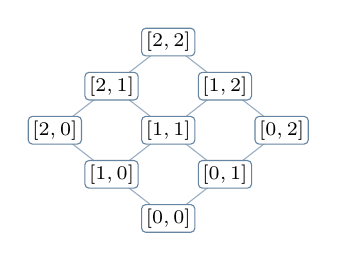
\begin{tikzpicture}[x=0.72cm, y=0.56cm,
  l/.style={draw=unimi!60, fill=white, rounded corners=1.5pt, inner sep=1.5pt, font=\scriptsize},
  e/.style={draw=unimi!40}]
  \foreach \a in {0,1,2} \foreach \b in {0,1,2} {
    \coordinate (c\a\b) at ({\b-\a},{\a+\b});
  }
  \foreach \a in {0,1,2} \foreach \b in {0,1} {
    \pgfmathtruncatemacro{\bb}{\b+1}
    \draw[e] (c\a\b) -- (c\a\bb);
    \draw[e] (c\b\a) -- (c\bb\a);
  }
  \foreach \a in {0,1,2} \foreach \b in {0,1,2} {
    \node[l] at (c\a\b) {$[\a,\b]$};
  }
\end{tikzpicture}
\column{0.5\textwidth}
\centering
\textbf{\color{unimi}Località geografica}\\[1mm]
{\small Località raggruppate in gruppi geografici\\[1.5mm]
$loc : \mathcal{N} \rightarrow \Omega$\\[1mm]
$\mathcal{G} \subseteq 2^{\Omega}$\\[1mm]
$geo : \mathcal{T} \cup \mathcal{D} \rightarrow \mathcal{G}$\par}
\vspace{2mm}
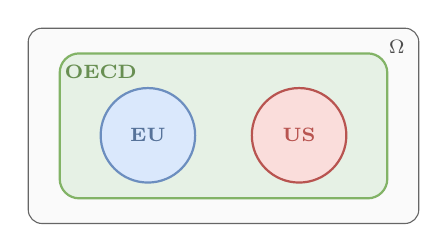
\begin{tikzpicture}[scale=0.8,
  gl/.style={font=\scriptsize\bfseries},
  pt/.style={circle, fill=black!70, inner sep=1.1pt}]
  \draw[rounded corners=5pt, fill=black!2, draw=black!60] (-3.1,-1.55) rectangle (3.1,1.55);
  \node[gl, text=black!70] at (2.75,1.25) {$\Omega$};
  \draw[thick, rounded corners=7pt, fill=diogreen!60, draw=diogreenborder] (-2.6,-1.15) rectangle (2.6,1.15);
  \node[gl, text=diogreenborder!80!black] at (-1.95,0.85) {OECD};
  \draw[thick, fill=dioblue, draw=dioblueborder] (-1.2,-0.15) circle (0.75);
  \node[gl, text=dioblueborder!80!black] at (-1.2,-0.15) {EU};
  \draw[thick, fill=diored!70, draw=dioredborder] (1.2,-0.15) circle (0.75);
  \node[gl, text=dioredborder] at (1.2,-0.15) {US};
\end{tikzpicture}
\end{columns}
\note{Slide di riserva sui nodi. $\alpha(n)$ è la classe di un nodo, con il livello più alto raggiunto per ogni proprietà, e $\beta$ è il livello minimo richiesto da task e dataset. Le classi formano un reticolo. Per la posizione, $loc$ dà la località di un nodo e $geo$ il gruppo geografico ammesso.}
\end{frame}

\begin{frame}{Riserva: politiche statiche}
\begin{center}
{\small
\begin{tabular}{@{}llll@{}}
\toprule
 & \textbf{Famiglia} & \textbf{Cosa garantisce} & \textbf{Vincolo} \\
\midrule
$c_{auth}$ & $\mathcal{C_A}$ & L'issuer è autorizzato sui dati & $ctx(d) \subseteq auth(iss(t))\ \ \forall d \in req(t)$ \\[1.5mm]
$c_{prop}$ & $\mathcal{C_T} \cap \mathcal{C_D}$ & Il nodo ha almeno i livelli richiesti & $\alpha(n) \succeq \beta^*(t)$ \\[1.5mm]
$c_{geo}$ & $\mathcal{C_T} \cap \mathcal{C_D}$ & Il nodo è in un'area ammessa & $loc(n) \in geo^*(t)$ \\[1.5mm]
$c_{static}$ & $\mathcal{C_D}$ & I dataset statici sono già sul nodo & $d \notin \mathcal{D}_{static} \lor n \in \lambda(d)\ \ \forall d \in req(t)$ \\
\bottomrule
\end{tabular}}
\end{center}
\vspace{2mm}
\begin{center}
\small
Il task \textbf{eredita} i requisiti dai dataset richiesti tramite:\\[2mm]
$\begin{aligned}
\beta^*(t) &= \beta(t) \sqcup \textstyle\bigsqcup_{d \in req(t)} \beta(d)\\[0.5mm]
geo^*(t) &= geo(t) \cap \textstyle\bigcap_{d \in req(t)} geo(d)
\end{aligned}$\\[2mm]
quindi, valendo per ogni dataset richiesto, $c_{prop},\, c_{geo} \in \mathcal{C_T} \cap \mathcal{C_D}$
\end{center}
\note{Slide di riserva con i vincoli formali delle quattro politiche statiche e con l'ereditarietà dei requisiti dai dataset al task, che permette di verificare $c_{prop}$ e $c_{geo}$ una volta sola sul task.}
\end{frame}

\begin{frame}{Riserva: formule degli indicatori}
\begin{columns}[T]
\column{0.47\textwidth}
\centering
\textbf{\color{unimi}Eccesso di proprietà}\\[3mm]
$\phi_{prop}(n,t) = 1 - \dfrac{\Delta(n,t)}{\Delta_{max}(t)}$\\[3mm]
{\small $\Delta(n,t) = \sum_{p \in \mathcal{P}} w_p\, \dfrac{\alpha_p(n) - \beta^*_p(t)}{\max \mathcal{L}_p - \beta^*_p(t)}$\\[2mm] $\Delta_{max}(t) = \sum_{p \in \mathcal{P}} w_p$}\\[3mm]
{\footnotesize\color{black!65} premia il nodo più vicino ai requisiti}
\column{0.47\textwidth}
\centering
\textbf{\color{unimi}Costo di trasferimento}\\[3mm]
$\phi_{transfer}(n,t) = 1 - \dfrac{size(remote(n,t))}{size(req(t))}$\\[3mm]
{\small $remote(n,t) = \{\, d \in req(t) \mid n \notin \lambda(d) \,\}$}\\[3mm]
{\footnotesize\color{black!65} premia il nodo con più dati già in locale}
\end{columns}
\vspace{6mm}
\begin{center}
\fcolorbox{unimi!40}{unimi!4}{\begin{minipage}{0.7\textwidth}\centering
$\mathcal{S}_\Phi(n,t) = w_{\phi_{prop}}\, \phi_{prop}(n,t) + w_{\phi_{transfer}}\, \phi_{transfer}(n,t)$
\end{minipage}}
\end{center}
\note{Slide di riserva con le formule degli indicatori. $\phi_{prop}$ vale 1 quando la classe del nodo coincide con i requisiti effettivi, e decresce con l'eccesso pesato, normalizzato da $\Delta_{max}$. $\phi_{transfer}$ vale 1 quando tutti i dataset richiesti sono già sul nodo.}
\end{frame}

\begin{frame}{Riserva: impostazione della valutazione}
\begin{columns}[c]
\column{0.44\textwidth}
{\small
\begin{tabular}{@{}ll@{}}
\toprule
Cluster kind & 5 nodi worker \\
Contesti & 10 \\
Task per run & 200, uno al secondo \\
Durata di un task & 20 s \\
Repliche & 5 per scenario \\
\bottomrule
\end{tabular}}
\vspace{3mm}

{\footnotesize Nodi omogenei: le politiche statiche restano attive ma non distinguono tra i nodi, quindi ogni ritardo è dovuto a $c_{wall}$.}
\column{0.52\textwidth}
\textbf{\color{unimi}Densità di conflitto $\rho$}\\
{\small Frazione di coppie di contesti in conflitto.\\Agisce sulla \emph{probabilità} che un task sia bloccato.}\\[4mm]
\textbf{\color{unimi}Intervallo di sanificazione $\tau$}\\
{\small Ogni quanto i nodi vengono ripuliti.\\Agisce sul \emph{tempo} che un task bloccato attende.}
\end{columns}
\msg{Metrica principale: latenza di scheduling, dalla sottomissione al binding.}
\note{Per la valutazione mi sono concentrato sulla politica dinamica, perché è l'unica il cui effetto cambia nel tempo. Le politiche statiche, per un dato task, o sono soddisfatte o non lo sono.

Ho usato un cluster kind con cinque nodi worker configurati in modo identico, così che ogni ritardo osservato sia attribuibile al Chinese Wall. Ogni run sottomette duecento task, uno al secondo, e ogni scenario è ripetuto cinque volte.

I fattori in gioco sono due. La densità di conflitto, cioè quante coppie di contesti sono in conflitto, incide sulla probabilità che un task venga bloccato. L'intervallo di sanificazione incide invece su quanto a lungo un task bloccato deve aspettare. Ho fatto due esperimenti, variando un fattore alla volta, e ho misurato soprattutto la latenza di scheduling.}
\end{frame}

% ===========================================================================
\begin{frame}{Riserva: la latenza cresce con i conflitti}
\begin{columns}[c]
\column{0.49\textwidth}
\centering
\includegraphics[width=0.86\linewidth]{immagini/val_conflitti/conflicts_latenza.jpg}\\
{\scriptsize Latenza media di scheduling ($\tau = 20$ s)}
\column{0.49\textwidth}
\centering
\includegraphics[width=0.86\linewidth]{immagini/val_conflitti/conflicts_grado.jpg}\\
{\scriptsize Task bloccati in funzione del grado del contesto}
\end{columns}
\vspace{2mm}
{\small Da 1.2 s a 15.6 s tra $\rho = 0.1$ e $\rho = 0.8$; task bloccati dal 20\% al 63\%. Crescita monotona (Spearman $r_s = 0.97$).}
\msg{A governare il blocco è il grado del contesto, più della densità.}
\note{Nel primo esperimento tengo fissa la sanificazione a venti secondi e faccio crescere la densità di conflitto.

A sinistra si vede che la latenza media cresce in modo monotono, da poco più di un secondo fino a quasi sedici. La ragione è che aumentano i task bloccati almeno una volta, che passano dal venti al sessantatré per cento.

Il grafico a destra spiega il perché. Sull'asse orizzontale c'è il grado del contesto, cioè con quanti altri contesti è in conflitto. Le curve delle diverse densità tendono a sovrapporsi: a parità di grado, un task viene bloccato più o meno con la stessa frequenza, qualunque sia la densità. Quindi non è la densità in sé a contare, ma il grado dei contesti, che la densità fa salire.}
\end{frame}

% ===========================================================================
\begin{frame}{Riserva: la sanificazione ha un intervallo ottimale}
\begin{columns}[c]
\column{0.49\textwidth}
\centering
\includegraphics[width=0.86\linewidth]{immagini/val_sanificazione/sanitize_latenza.jpg}\\
{\scriptsize Latenza media di scheduling ($\rho = 0.5$)}
\column{0.49\textwidth}
\centering
\includegraphics[width=0.86\linewidth]{immagini/val_sanificazione/sanitize_disponibilita.jpg}\\
{\scriptsize Tempo in cui un nodo è indisponibile perché in sanificazione}
\end{columns}
\vspace{2mm}
{\small Andamento a U: circa 10 s a $\tau = 1$, minimo di 5.8 s a $\tau = 10$, oltre 23 s a $\tau = 50$. Regione ottimale tra 10 e 20 s, vicina alla durata dei task.}
\msg{Troppo spesso: nodi sempre in pulizia. Troppo di rado: tracce persistenti.}
\note{Nel secondo esperimento fisso la densità a zero virgola cinque e vario l'intervallo di sanificazione da uno a cinquanta secondi.

Qui l'andamento non è monotono ma a U. Con un intervallo molto breve la latenza è alta, scende fino a un minimo di circa sei secondi intorno a dieci, poi risale oltre i venti.

I due bracci hanno cause diverse. A sinistra si sanifica così spesso che i nodi passano la maggior parte del tempo in pulizia: lo mostra il grafico a destra, dove a un secondo i nodi sono indisponibili per oltre il novanta per cento del tempo. A destra invece si sanifica di rado, e le tracce in conflitto restano sui nodi troppo a lungo.

I test statistici dicono che l'ottimo non è un valore singolo, ma una regione tra dieci e venti secondi, che per questo carico coincide più o meno con la durata dei task.}
\end{frame}

% ===========================================================================
\begin{frame}{Riserva: test statistici}
\relax{\small
\begin{tabular}{@{}p{0.42\textwidth}ll@{}}
\toprule
\textbf{Confronto} & \textbf{Test} & \textbf{Esito} \\
\midrule
Effetto di $\rho$ sulla latenza & Kruskal-Wallis & $H = 37.08$, $p < 10^{-5}$ \\
Monotonia rispetto a $\rho$ & Spearman & $r_s = 0.97$, $p < 10^{-24}$ \\
\midrule
Effetto di $\tau$ sulla latenza & Kruskal-Wallis & $H = 31.87$, $p < 10^{-4}$ \\
$\tau = 10$ contro $\tau = 5$ & Mann-Whitney & $U = 0$, $p < 10^{-2}$ \\
$\tau = 10$ contro $\tau = 20$ & Mann-Whitney & $U = 9$, $p = 0.90$ \\
$\tau = 20$ contro $\tau = 30$ & Mann-Whitney & $U = 1$, $p = 0.03$ \\
\bottomrule
\end{tabular}}
\vspace{4mm}

{\small Test condotti sulle latenze medie delle singole repliche. Tra $\tau = 10$ e $\tau = 20$ le prestazioni non sono distinguibili: l'ottimo è una regione, non un punto.}
\note{Slide di riserva, da usare solo se chiedono dei test statistici.}
\end{frame}

\begin{frame}{Riserva: cause di blocco}
\begin{columns}[c]
\column{0.49\textwidth}
\centering
\includegraphics[width=0.86\linewidth]{immagini/val_conflitti/conflicts_cause_blocco.jpg}\\
{\scriptsize Al variare di $\rho$}
\column{0.49\textwidth}
\centering
\includegraphics[width=0.86\linewidth]{immagini/val_sanificazione/sanitize_cause_blocco.jpg}\\
{\scriptsize Al variare di $\tau$}
\end{columns}
\vspace{2mm}
{\small \emph{none}: assegnati al primo tentativo. \emph{taint}: nodo in sanificazione. \emph{mixed}: traccia in conflitto e poi sanificazione. Con $\tau$ fisso i blocchi da solo \emph{taint} non crescono con $\rho$; con $\tau$ piccolo diventano una quota rilevante.}
\note{Slide di riserva sulle cause di blocco.}
\end{frame}

\begin{frame}{Riserva: limiti della valutazione}
\relax{\small
\begin{itemize}
\item \textbf{Task simulati}: non saturano CPU o memoria. In Kubernetes la capacità residua è già gestita dal plugin nativo \texttt{NodeResourcesFit}, esterno alle politiche della tesi.\\[2mm]
\item \textbf{Cluster su una sola macchina}: i valori assoluti di latenza non rappresentano un cluster di produzione. Contano gli andamenti.\\[2mm]
\item \textbf{Intervalli lunghi}: una run copre pochi cicli di pulizia, la varianza è alta e i valori oltre l'ottimo vanno letti come tendenza.\\[2mm]
\item \textbf{Sola sanificazione periodica}: la regione ottimale dipende dal carico, non è un valore universale.
\end{itemize}}
\note{Slide di riserva: perché ho valutato solo il Chinese Wall e quanto valgono i numeri su kind.}
\end{frame}

\begin{frame}{Riserva: come migliorare la sanificazione}
\begin{columns}[t]
\column{0.47\textwidth}
\textbf{\color{unimi}Combinare le strategie}\\[1mm]
{\small \textbf{Opportunistica}: pulisce un nodo appena è libero da task. Attenua il braccio sinistro della U.\\[2mm]
\textbf{A soglia}: pulisce quando $|\Lambda(n)|$ supera un limite, prima che il nodo si saturi.}
\column{0.47\textwidth}
\textbf{\color{unimi}Pulizia parziale}\\[1mm]
{\small Il nodo resta candidabile. Si attendono solo i task che stanno per finire, la traccia di quelli lunghi resta e blocca i soli task in conflitto.\\[2mm]
Richiede una stima della durata, che oggi i task black-box non offrono.}
\end{columns}
\note{Slide di riserva sugli sviluppi della sanificazione.}
\end{frame}

\begin{frame}{Riserva: il ciclo di scheduling}
\relax{\small
\begin{tabular}{@{}llp{0.52\textwidth}@{}}
\toprule
\textbf{Fase} & \textbf{Plugin} & \textbf{Cosa fa} \\
\midrule
Filter & WallFilter & Verifica $c_{wall}$ su ogni nodo candidato \\
PreScore & TransferScore & Una sola richiesta al dataset-service \\
Score & PropScore, TransferScore & Calcola $\phi_{prop}$ e $\phi_{transfer}$ \\
Reserve & WallFilter & Registra $ctx^*(t)$ in memoria, in modo sincrono \\
PostBind & WallFilter & $\Lambda(n) \leftarrow \Lambda(n) \cup ctx^*(t)$ sul nodo scelto \\
\bottomrule
\end{tabular}}
\vspace{4mm}

{\small La memoria si aggiorna solo sul nodo effettivamente scelto, non su quelli valutati. \emph{Reserve} copre la finestra in cui il binding, asincrono, non ha ancora reso visibile l'aggiornamento.}
\note{Slide di riserva sui dettagli dei plugin dello scheduler.}
\end{frame}

\fi
\setcounter{framenumber}{\value{ultimaslide}}
\end{document}